\section{Integracja systemu}

Ostatecznym etapem projektu było połączenie stworzonych w~ten sposób modułów w~ramach pojedynczego bloku języka VHDL. Ze względu na regularne testowanie wdrażanych elementów oraz z~góry przemyślaną strukturę projektu proces ten przebiegł bezpoleśnie. Ostatecznie projekt udało się zsyntezować, czego efekt przedstawia Rys. \ref{synthesis}.

\vspace{0.5cm}
\begin{figure}[ht]
    \centering
    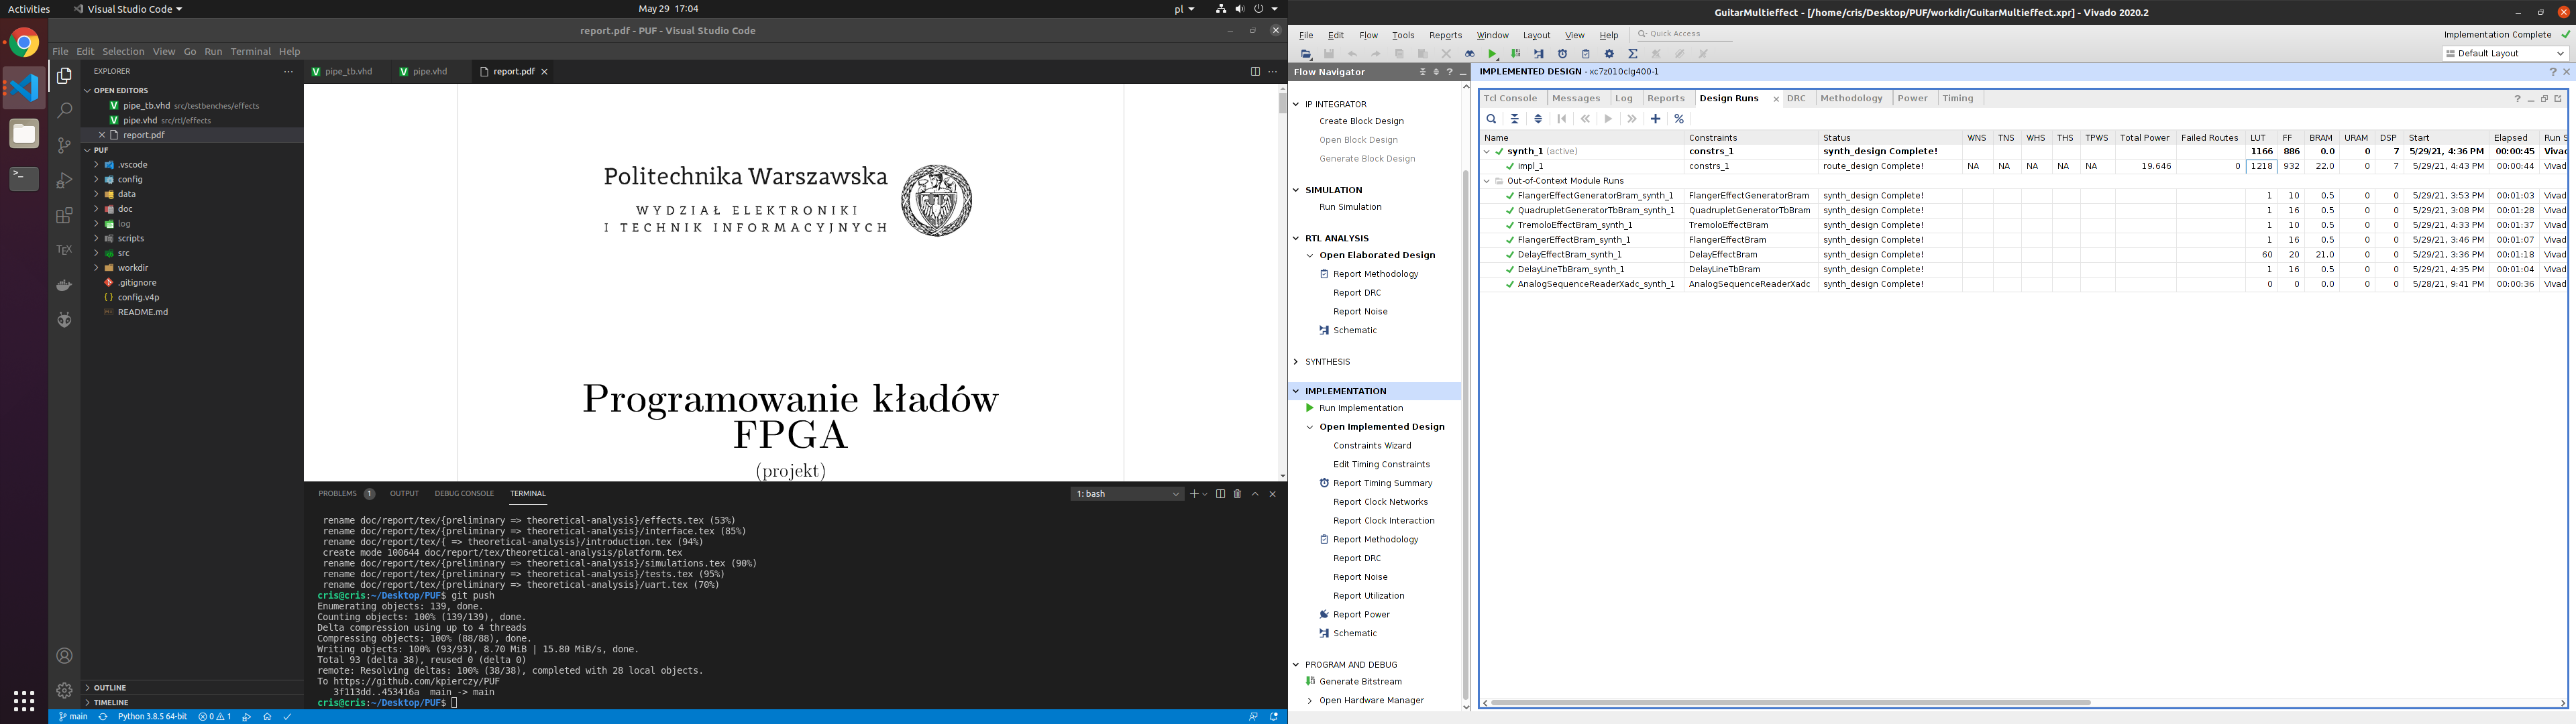
\includegraphics[width=\textwidth]{img/implementation.png}
    \captionsetup{format=plain,justification=centering}
    \caption{Efekt syntezy projektu}
    \label{synthesis}
\end{figure}
\vspace{0.5cm}

Niestety możliwość wykonania testów integracyjnych z~wykorzystaniem symulacji była dość ograniczona w~przypadku kompletnego projektu. Wynika to z~faktu, że oparametry wszytskich efektów określane są przez wartości pobierane przez interfejs analogowy z~\textbf{pojedynczego} kanału. Przezwyciężenie tej trudności wymagałoby zmodyfikowania skryptu generującego plik z~przebiegami sygnałów analogowych w~taki sposób, aby uzględniał czasy próbkowania przetwornika ADC i~zapisywał wartości napięcia odpowiadające aktualnie odczytywanego parametru. Ze względu na i~tak już szeroki zakres projektu zrezygnowano z~realizji takiego podejścia.
